\documentclass[12pt,a4paper,twoside]{article}
\usepackage{labor}
\begin{document}

%fill for cover and header creation
\newcommand\laboratorynumber{2}
\title{Halbleiterdiode}
\newcommand\supervisor{Ditlbacher, Harald}
\newcommand\groupnumber{42}

\newcommand\participantonelastname{Eisner}
\newcommand\participantonefirstname{Nico}
\newcommand\participantoneid{12214121}
\newcommand\participanttwolastname{Waldl}
\newcommand\participanttwofirstname{Philip}
\newcommand\participanttwoid{12214120}
\author{\participantonelastname \ \& \participanttwolastname}

\newcommand\degreeid{UB 033 678}
\newcommand\semester{23WS}
\date{15.12.2023}

%select correct course title
%\newcommand\coursetitle{Einführung in die \\ physikalischen Messmethoden}
%\newcommand\coursetitle{Laborübungen 1: \\ Mechanik und Wärme}
\newcommand\coursetitle{Laborübungen 2: \\ Elektrizität, Magnetismus, Optik}
%\newcommand\coursetitle{Fortgeschrittenen Praktikum 1: \\ Technische Physik}
%\newcommand\coursetitle{Fortgeschrittenen Praktikum 2: \\ Allgemeine Physik}

%\begin{titlepage}
   \begin{center}
       \begin{figure}[H]
            \begin{minipage}[h]{30mm}
                \centerline{
\includegraphics[height=15mm]{cover_nudes/tugraz.png}}
            \end{minipage}
            \hfill
            \begin{minipage}[h]{30mm}
                \centerline{
\includegraphics[height=15mm]{cover_nudes/nawi_graz.png}}
            \end{minipage}
            \hfill
            \begin{minipage}[h]{30mm}
                \centerline{
\includegraphics[height=15mm]{cover_nudes/uni-graz.png}}
            \end{minipage}
        \end{figure}
        
        \large{\emph{Institut für Experimentalphysik der Technischen Universität Graz \\
        \& Institut für Physik der Universität Graz}} \\
        \vspace{5mm}
        
        {\Huge \textbf{\coursetitle}}
        \vspace{5mm}
        
        {\huge \laboratorynumber: \thetitle}
    \end{center}
    
    \vfill
    
    \begin{table}[H]
        \LARGE
        \centering
        \begin{tabular}{r l}
            Betreuer:       & \supervisor \\
            Gruppennummer:  & \groupnumber \\
            \\
            Name:           & \participantonelastname, \participantonefirstname \\
            Matrikelnummer: & \participantoneid \\
            Name:           & \participanttwolastname, \participanttwofirstname \\
            Matrikelnummer: & \participanttwoid \\
            \\
            Kennzahl:       & \degreeid \\
            Datum:          & \semester \ | \thedate
        \end{tabular}
    \end{table}
    \vspace{4cm}
\end{titlepage}
\clearpage
\setcounter{page}{1}

%\maketitle %short title alternative

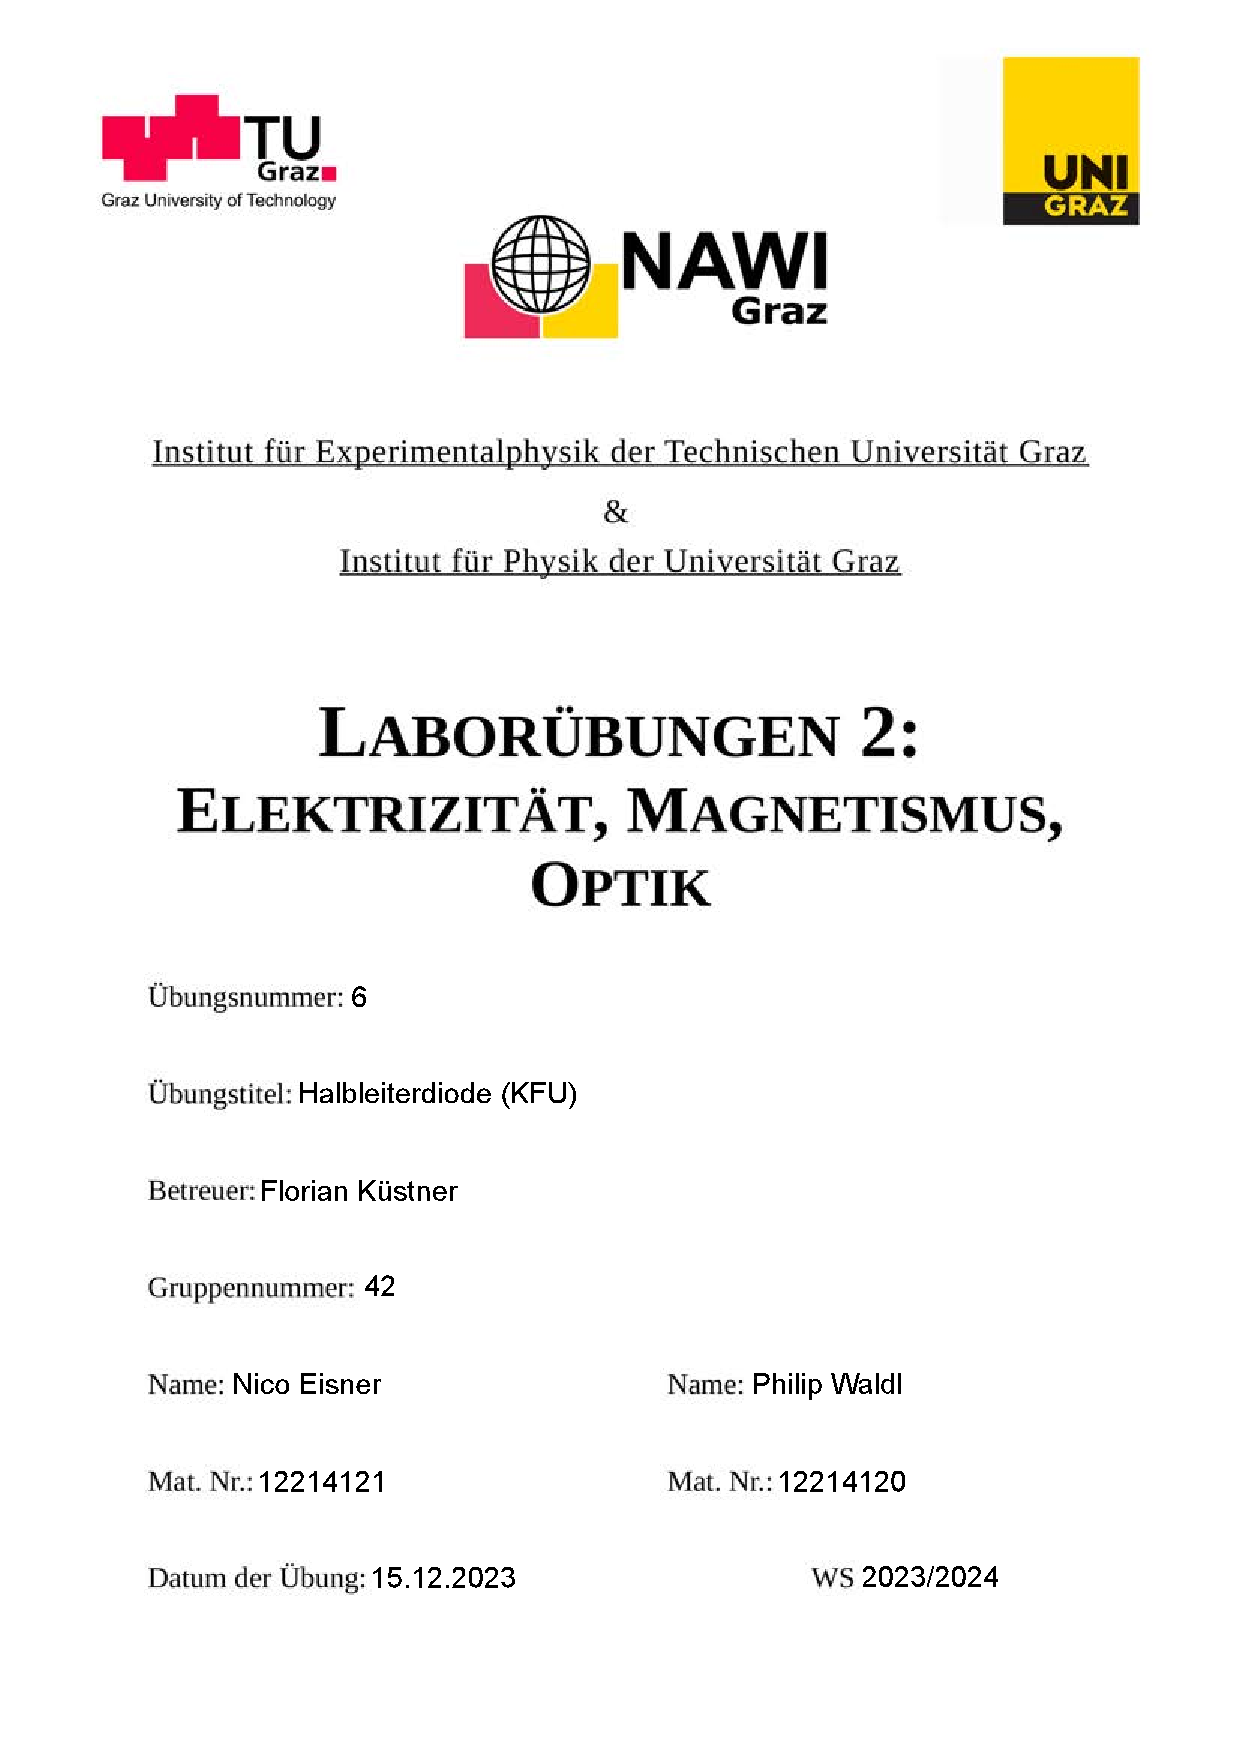
\includepdf[pages={1}]{../Deckblätter/Deckblatt_Halbleiterdiode.pdf}

\tableofcontents
\newpage

\section{Aufgabenstellung} %jo beschreibn wos gmocht host ------------------------------
Das Experiment Halbleiterdiode besteht aus drei Teilaufgaben. 
\\
In der ersten Teilaufgabe gilt es die Strom-Spannungs Charakteristik einer Gleichrichterdiode in Durchlassrichtung sowie in Sperrrichtung zu bestimmen. 
\\
Im zweiten Teil wird die Strom-Spannungs Charakteristik einer Zenerdiode in Durchlassrichtung und Sperrrichtung bestimmt. 
\\
Im dritten und letzten Teil werden Spannungs- und Stromverläufe in einer Einweg- Gleichrichterschaltung mit unterschiedlichen Glättungskondensatoren sowie mit Belastungswiderständen untersucht. 
\\
\\
Alle Informationen und Methodiken wurden uns von der Technischen Universität bereitgestellt \cite{teachcenter2}. 


\section{Voraussetzungen \& Grundlagen} %Grundlagen erklären, Formeln mit erklärung
Um mit dem Experiment beginnen zu können gilt es erst zu erklären, was ein Halbleiter ist. 
\\
Es gibt drei arten der elektrischen Leitfähigkeit. Leitern, Nichtleitern und Halbleitern. Mithilfe des quantenmechanischen Bändermodells lässt sich die Leitfähigkeit beschreiben. 
Dieses besteht aus den zwei Energiebändern (Leitungsband und Valenzband) und der Bandlücke. Valenzelektronen befinden sich im Valenzband und dienen als Ladungsträger. Im Grundzustand ist das Leitungsband nicht mit Elektronen besetzt. 
Zwischen diesen befindet sich bei Halbleitern und Nichtleitern die Bandlücke. 

\begin{figure}[H]
    \centering
    \includegraphics[width=0.6\linewidth,]{nudes/bändermodell.jpg}
    \caption{Bändermodell eines Nichtleiters, Halbleiters und Leiters. Entnommen aus Skriptum Halbleiterdiode Abbildung 7. \cite{teachcenter2}}
    \label{fig:Bändermodell}
\end{figure}

\noindent
Bei Leitern existiert keine Bandlücke. Das Valenzband ist nicht voll mit Elektronen besetzt oder es überlappt mit dem Leitungsband. Diese Zustände treffen gleichzeitig zu. 
Bei Nichtleitern ist zwischen Valenzband und Leitungsband die Bandlücke. Das Valenzband ist voll mit Elektronen, diese können aber nicht zum Leitungsband gelangen. 
Bei Halbleitern ist die Bandlücke sehr klein im Gegensatz zu Nichtleitern. Bei Raumtemperatur können Elektronen vom Valenzband in das Leitungsband gelangen. 
Dadurch hinterlässt jedes in das Leitungsband übergetretene Elektron ein Loch, welches durch andere Elektronen besetzt wird. 
\\
Da die Elektronen aber wieder in dieses Loch zurückfallen würden, ist die Eigenleitfähigkeit dieser Halbleiterelemente nicht verwertbar. 
\\
\\
Durch das einbringen fremder Atome in den Halbleiterkristall lässt sich die Leitfähigkeit ändern. Halbleiter bestehen meißt aus Silizium oder Germanium. 
Bei Silizium handelt es sich um 4-wertige Valenzelelektronen. Durch einbringen eines 3-wertigen oder 5-wertigen Atomes lässt sich die Leitfähigkeit gezielt verändern. 

\begin{figure}[H]
    \centering
    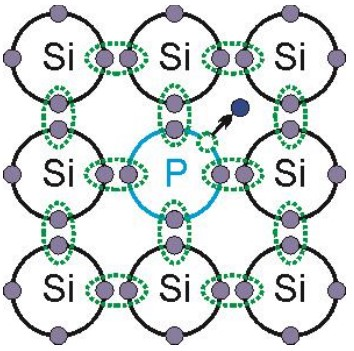
\includegraphics[width=0.3\linewidth,]{nudes/n-dot.jpg}
    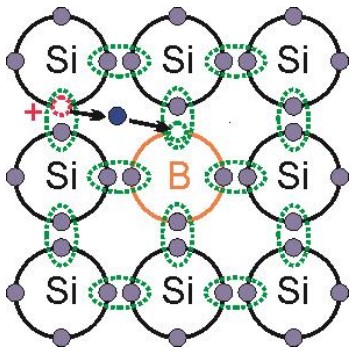
\includegraphics[width=0.3\linewidth,]{nudes/p-dot.jpg}
    \caption{n-Dotierter Kristall (links) und p-Dotierter Kristall (rechts). Bei dem n-Dotierten Kristall wird Phosphor eingebracht und bei dem p-Dotierten wird Bor eingebracht. Entnommen aus Skriptum Halbleiterdiode Abbildung 8 und 9. \cite{teachcenter2}}
    \label{fig:n und p dotiert}
\end{figure}

\noindent
Bringt man in die Kristallstruktur ein 5-wertiges Dotierelement ein, so spricht man von n-Dotierung. Dieses fünfte Elektron ist dabei frei beweglich. 
Bringt man ein 3-wertiges Dotierelement ein, so spricht man von p-Dotiertung. Dieses entstandene Loch kann ein Außenelektron aufnehmen. 
Bei einen pn-Übergang ist dies genau der Fall. Dieser ist der Übergangsbereich unterschiedlich dotierter Halbleiterkristalle. 
Elektronen des n-Kristalls wandern zuu den Löchern des p-Kristalls. Löcher des p-Kristalls wandern zu den Elektronen des n-Kristalls. 
Durch diesen Vorgang entsteht ein elektrisches Feld. Der Halbleiter ist nichtmehr elektrisch neutral und die Kraft, welche das el. Feld erzeugt wirkt auf die verbleibenden Ladungsträger. 
\\
\\
Verpackt man eine p-n Übergang in ein Gehäuse und versorgt ihn mit Anschlüssen erhält man eine Diode. 

\begin{figure}[H]
    \centering
    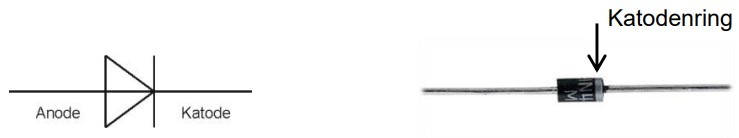
\includegraphics[width=0.6\linewidth,]{nudes/diode.jpg}
    \caption{Schaltbild und Foto einer Diode. Entnommen aus Skriptum Halbleiterdiode Abbildung 15. \cite{teachcenter2}}
    \label{fig:Diode}
\end{figure}

\begin{equation}
    \label{eq:Müll}
    \centerline{$M=\frac{muell}{malle}$}
\end{equation}

\section{Versuchsanordnung} %mit skizze kurz beschreiben ------------------------------
Der Versuch wird auf dem Steckbrett aufgebaut und durch mehrere Messgeräte wie Multimeter und Oszilloskope ergänzt. 

\begin{figure}[H]
    \centering
    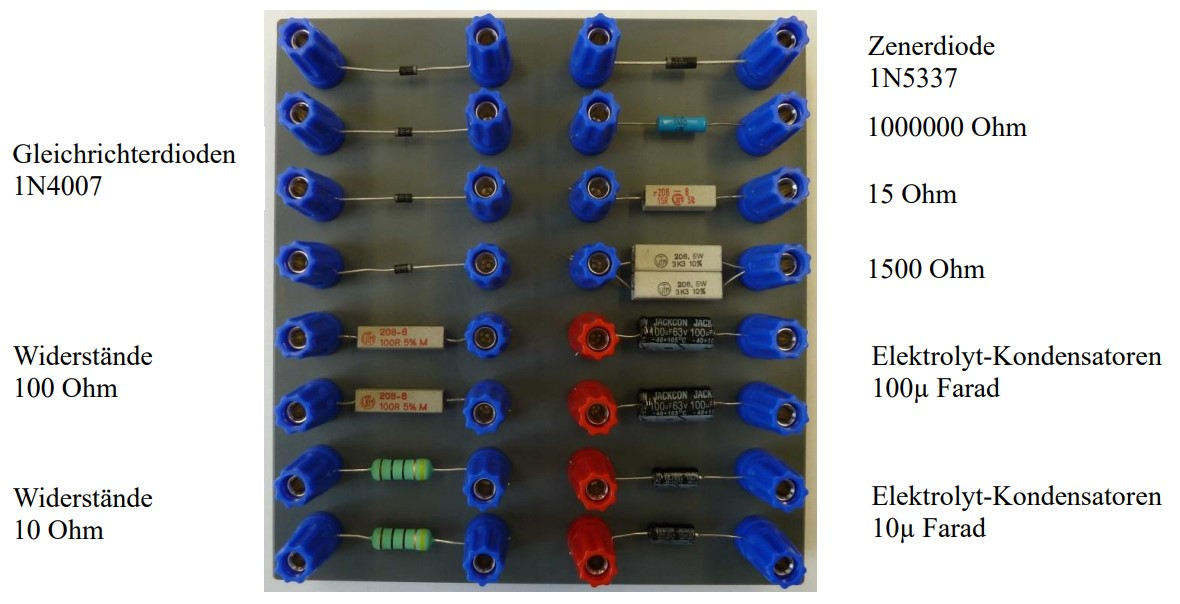
\includegraphics[width=0.6\linewidth]{nudes/steckbrett.jpg}
    \caption{Steckbrett mit Bauteilen. Entnommen aus Skriptum Halbleiterdiode Abbildung 1. \cite{teachcenter2}}
    \label{fig:Steckbrett}
\end{figure}

\subsection{Teil 1}
Im ersten Teil wird die Strom-Spannungskennlinie der Gleichrichterdiode in Durchlassrichtung bestimmt. Der Aufbau sieht dabei wiefolgt aus. 

\begin{figure}[H]
    \centering
    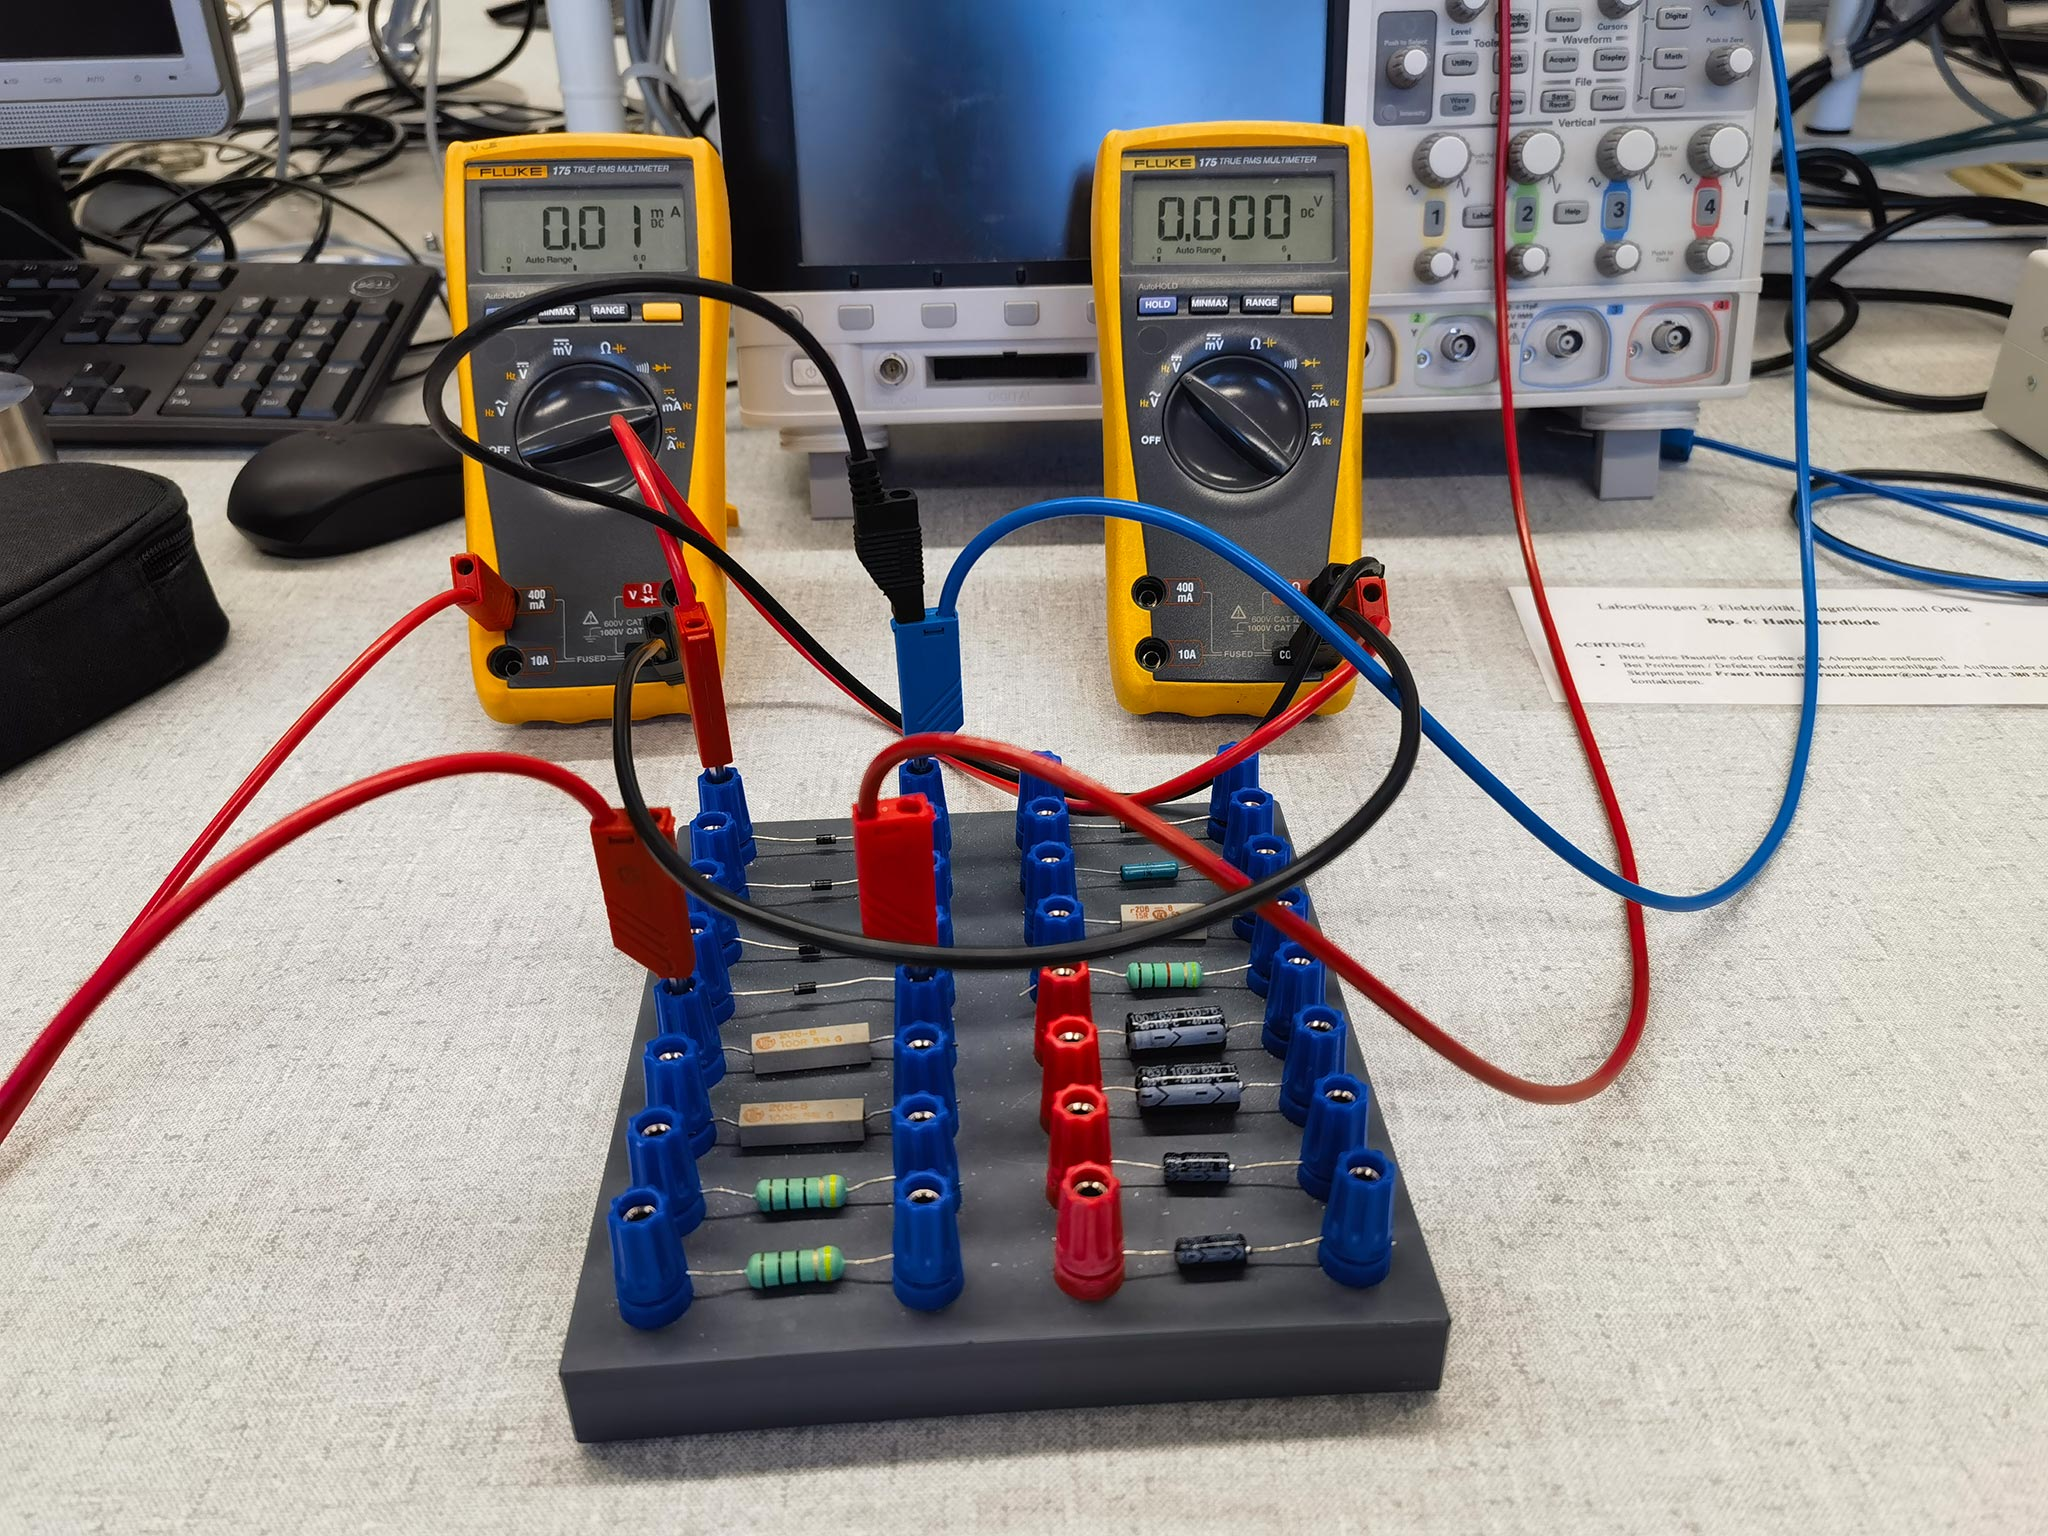
\includegraphics[width=0.4\linewidth]{nudes/1a.jpg}
    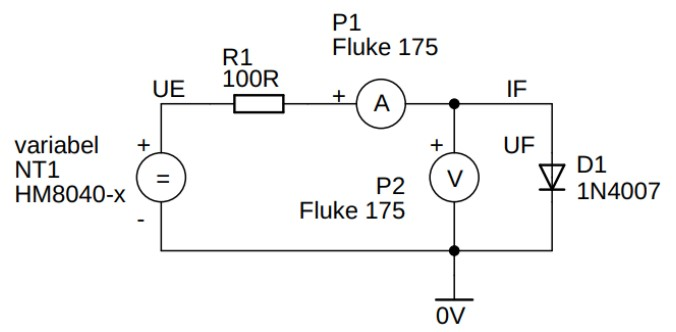
\includegraphics[width=0.4\linewidth]{nudes/aufbau1a schaltplan.jpg}
    \caption{Schaltbild (links) und Aufbau (rechts) Teil 1. Schaltbild entnommen aus Skriptum Halbleiterdiode Abbildung 1. \cite{teachcenter2}}
    \label{fig:aufbau 1a}
\end{figure}

\noindent
Das gleiche wird anschließend für die Gleichrichterdiode in Sperrichtung wiederholt.

\begin{figure}[H]
    \centering
    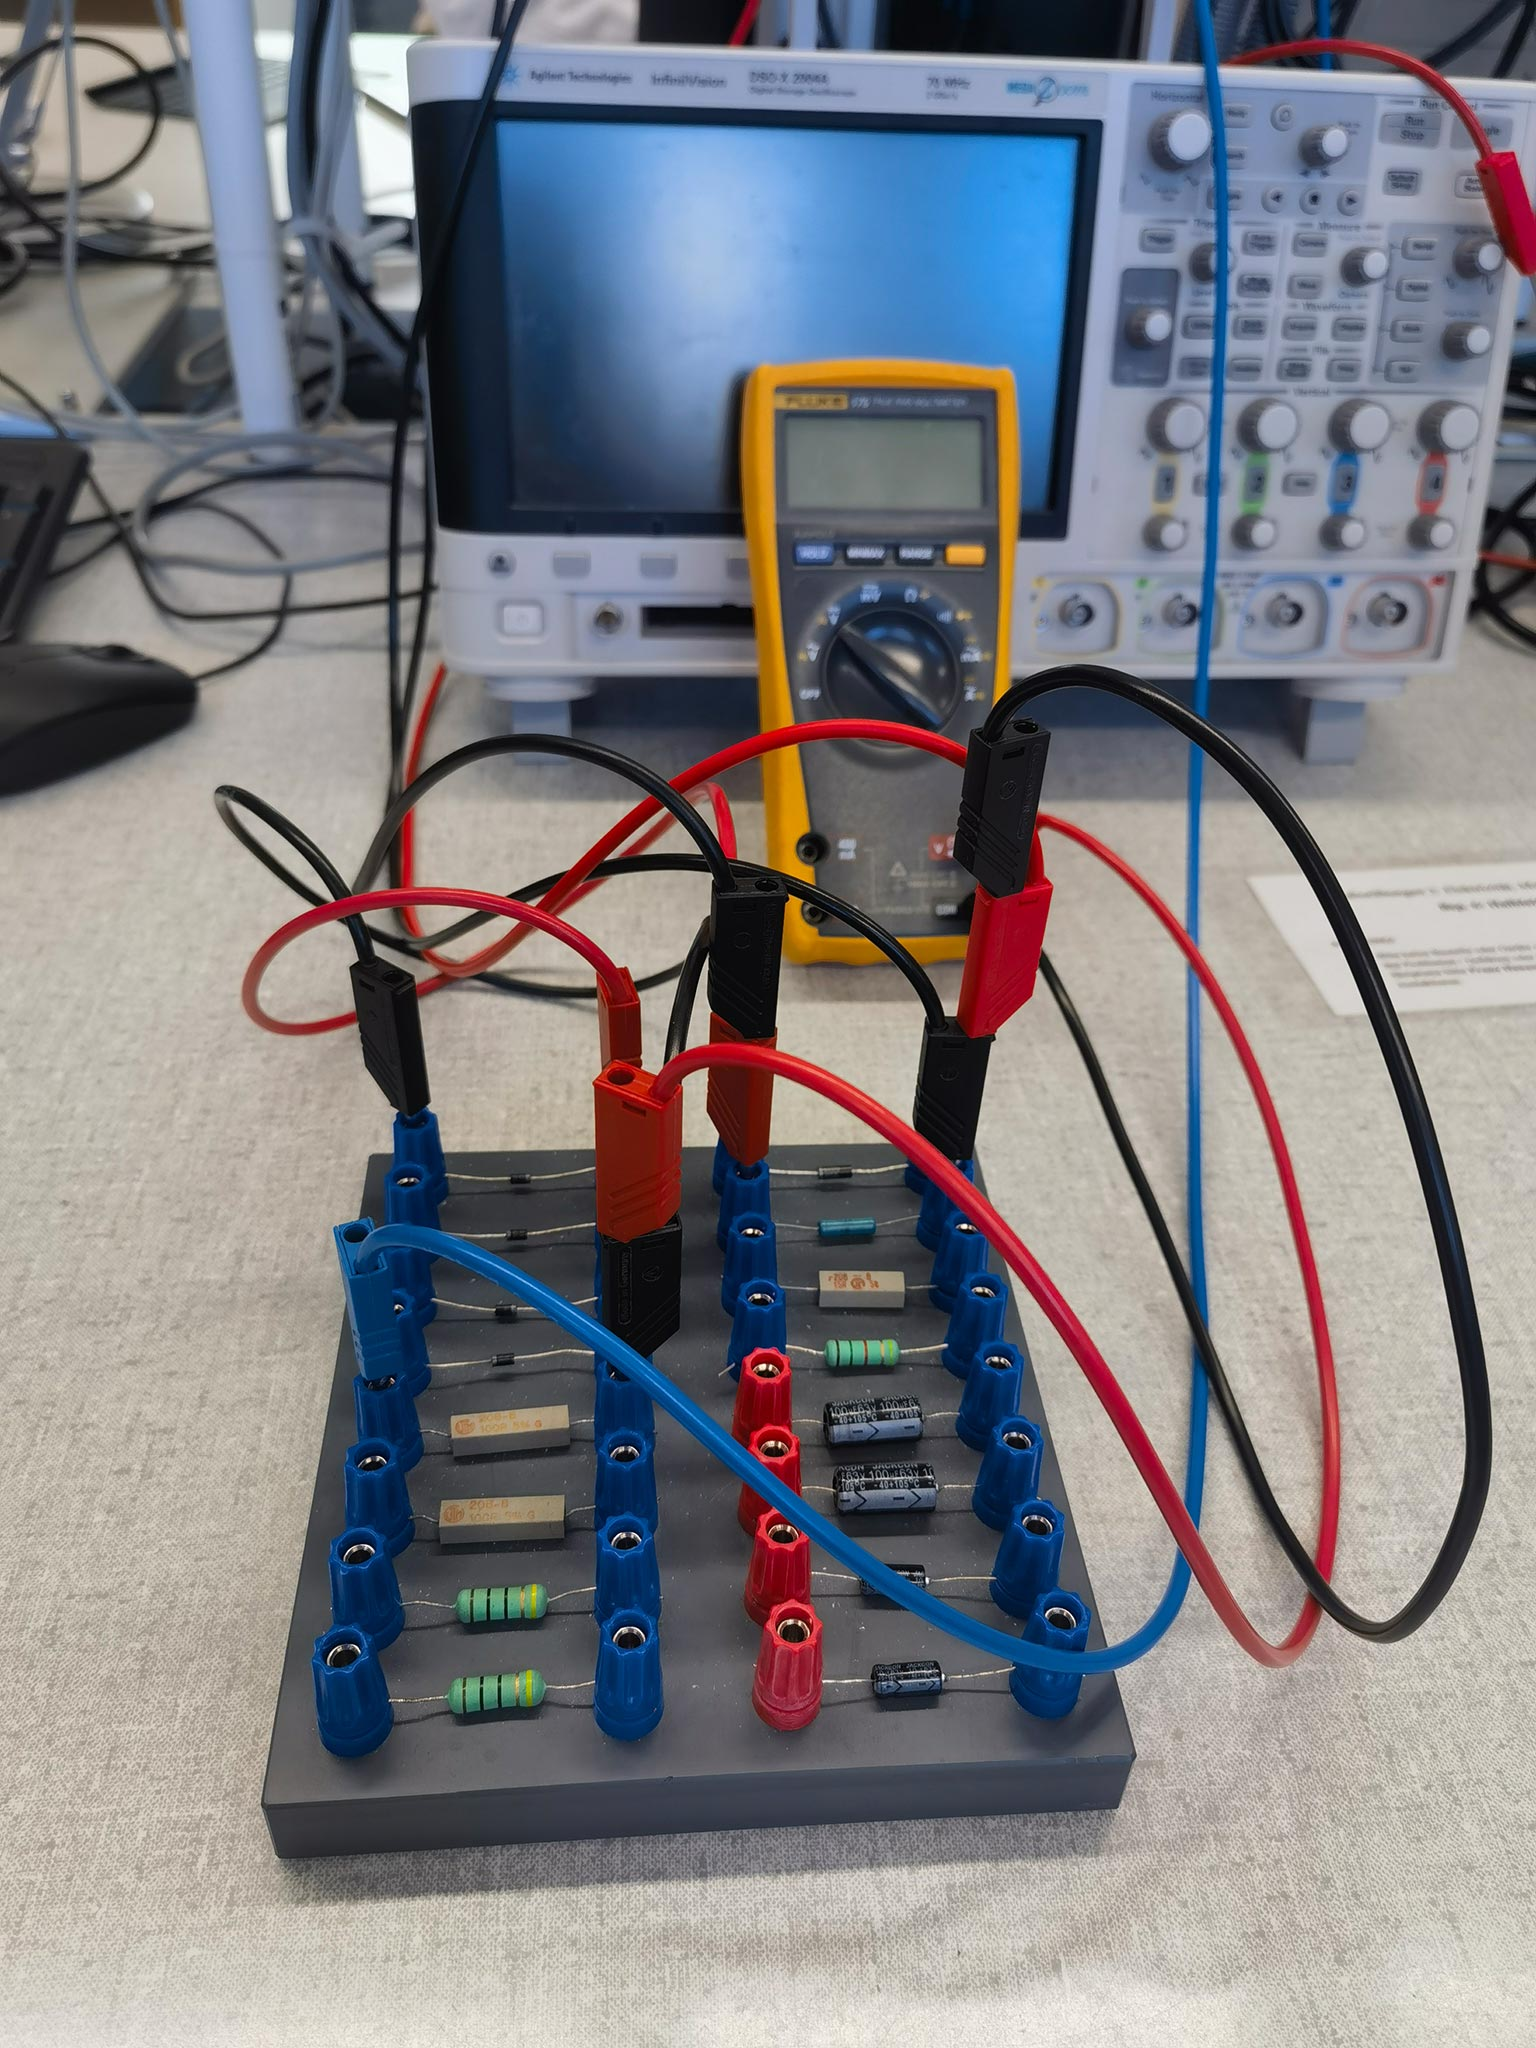
\includegraphics[width=0.4\linewidth]{nudes/1b.jpg}
    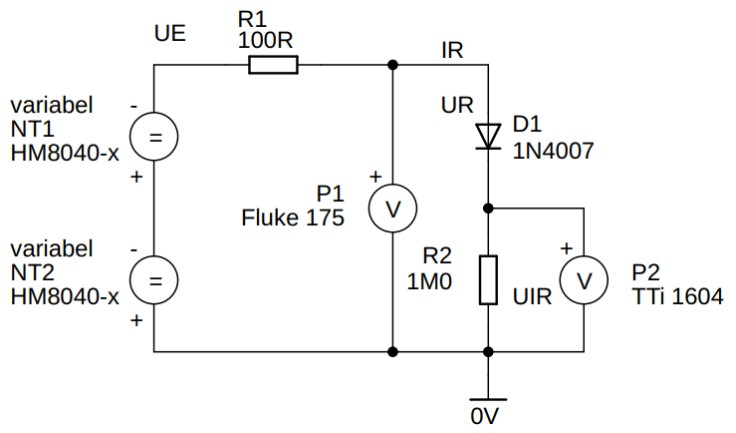
\includegraphics[width=0.4\linewidth]{nudes/aufbau1b schaltplan.jpg}
    \caption{Schaltbild (links) und Aufbau (rechts) Teil 1. Schaltbild entnommen aus Skriptum Halbleiterdiode Abbildung 1. \cite{teachcenter2}}
    \label{fig:aufbau 1b}
\end{figure}

\subsection{Teil 2}
Im zweiten Teil wird die Strom-Spannungskennlinie einer Zenerdiode aufgenommen. 

\begin{figure}[H]
    \centering
    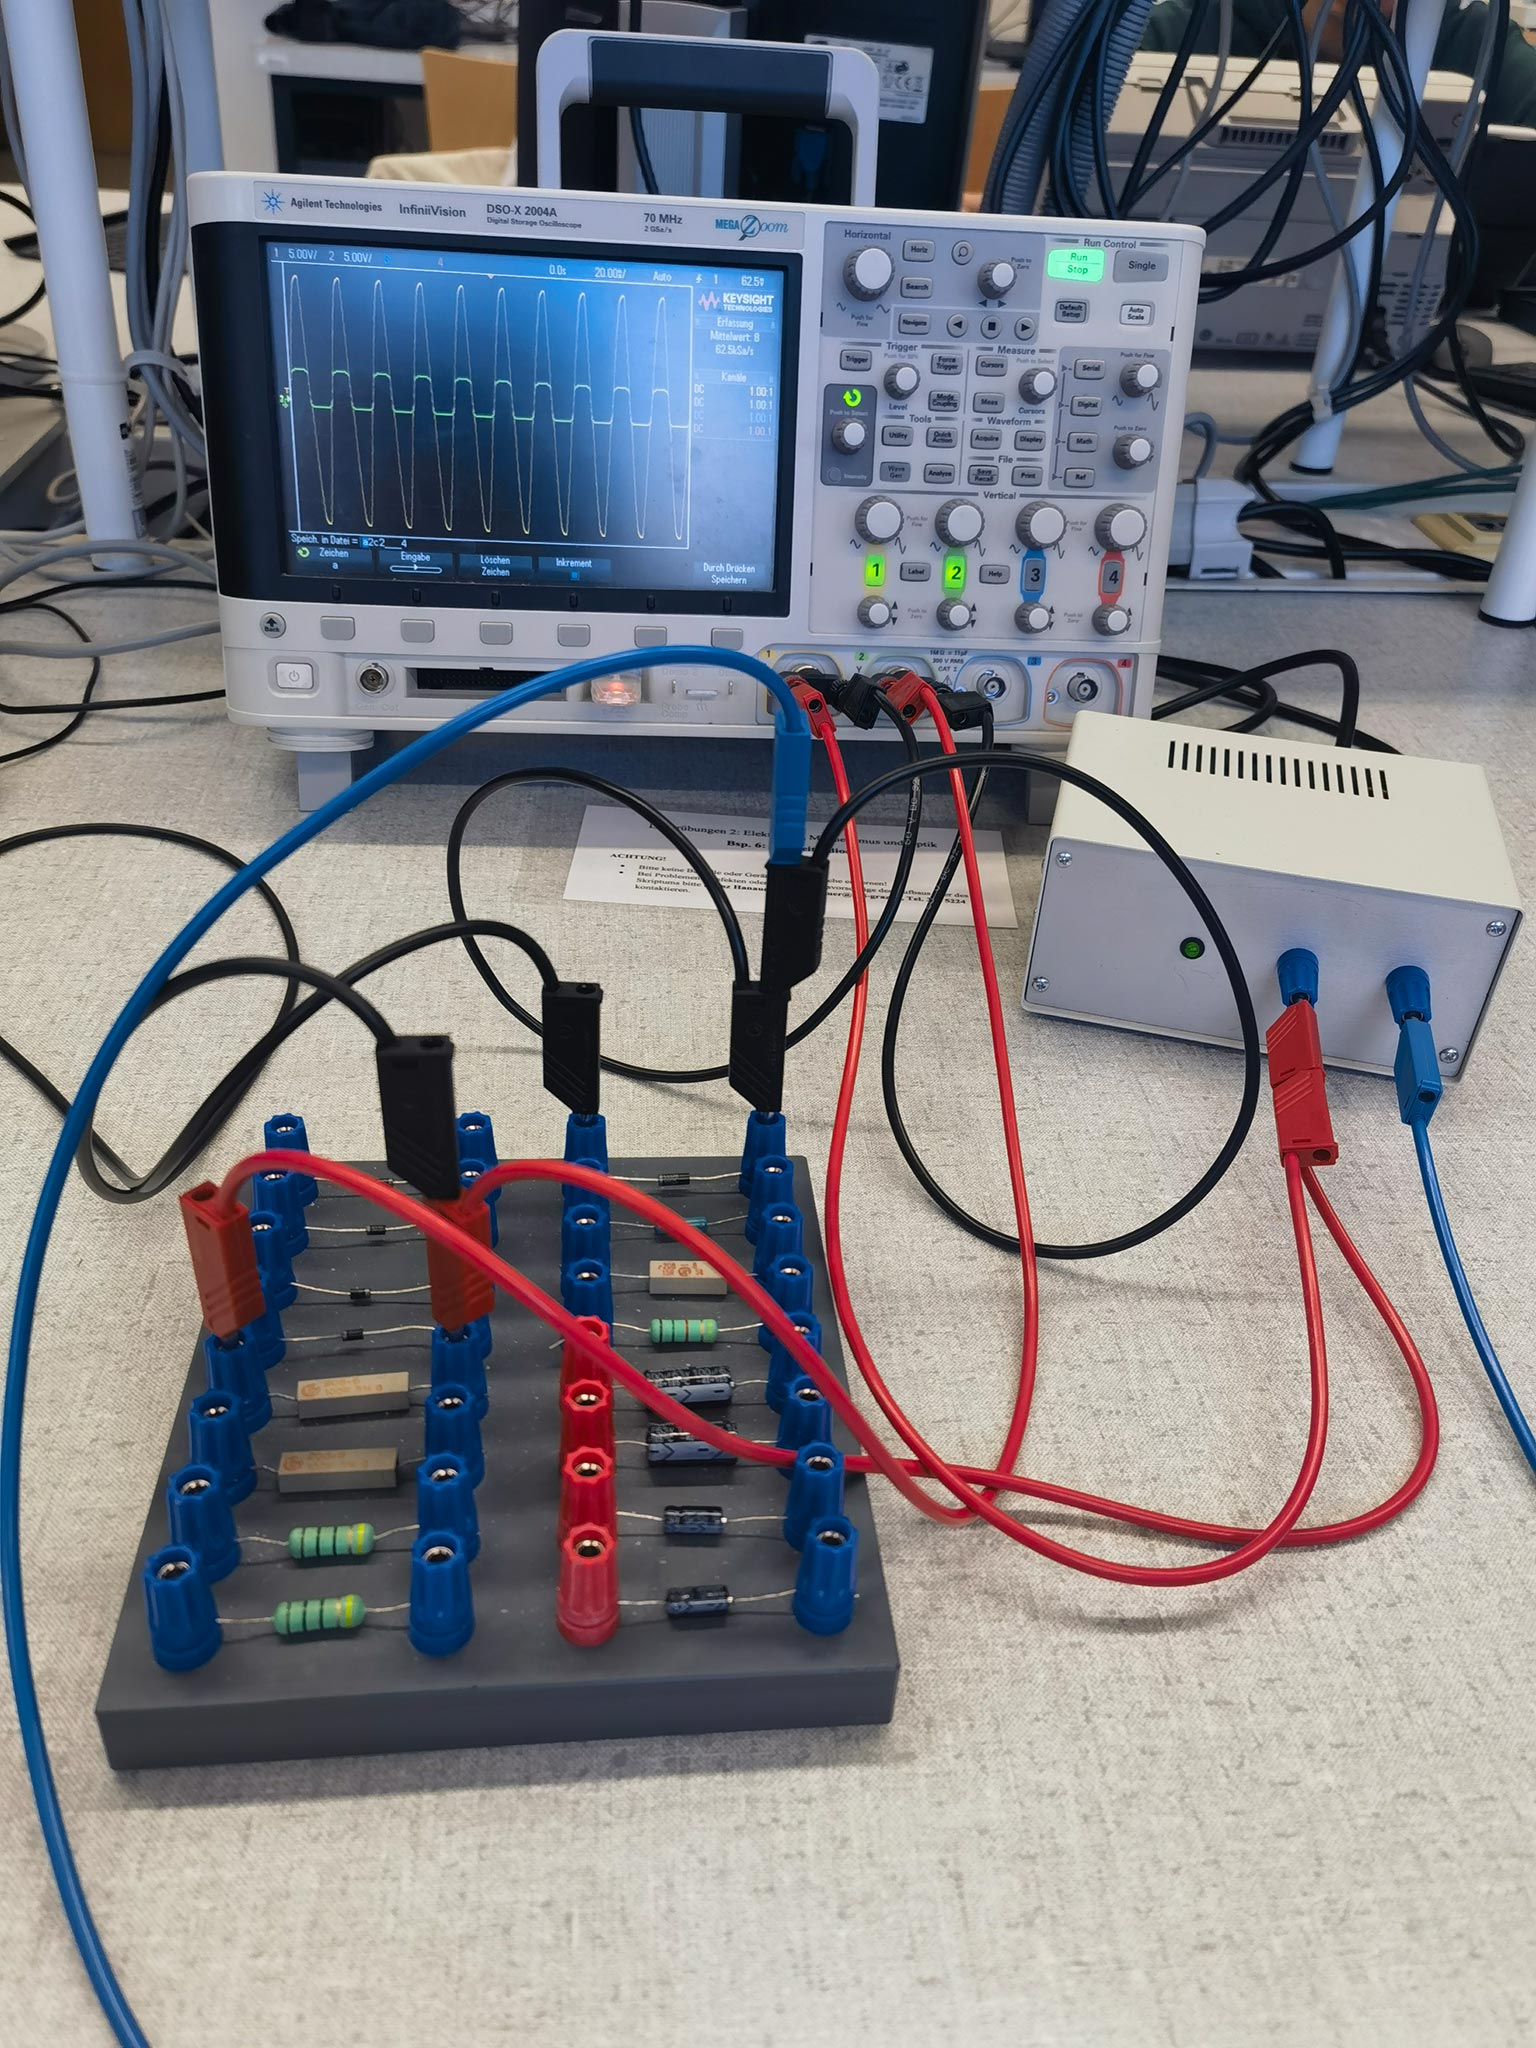
\includegraphics[width=0.4\linewidth]{nudes/2.jpg}
    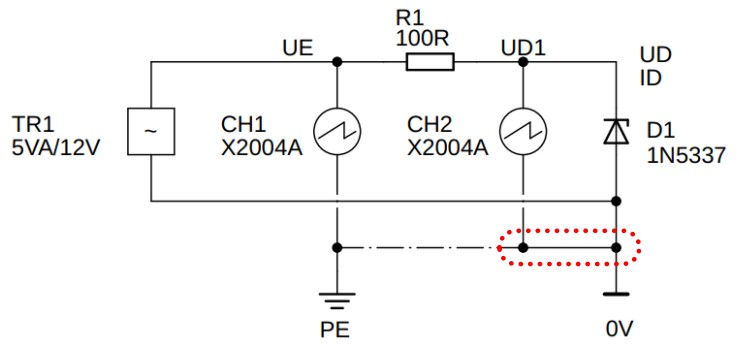
\includegraphics[width=0.4\linewidth]{nudes/aufbau2 schaltplan.jpg}
    \caption{Schaltbild (links) und Aufbau (rechts) Teil 2. Schaltbild entnommen aus Skriptum Halbleiterdiode Abbildung 1. \cite{teachcenter2}}
    \label{fig:aufbau 2}
\end{figure}

\subsection{Teil 3}
Im dritten Teil wird die grafische Darstellung der Verläufe von Strom und Spannung bestimmt. 

\begin{figure}[H]
    \centering
    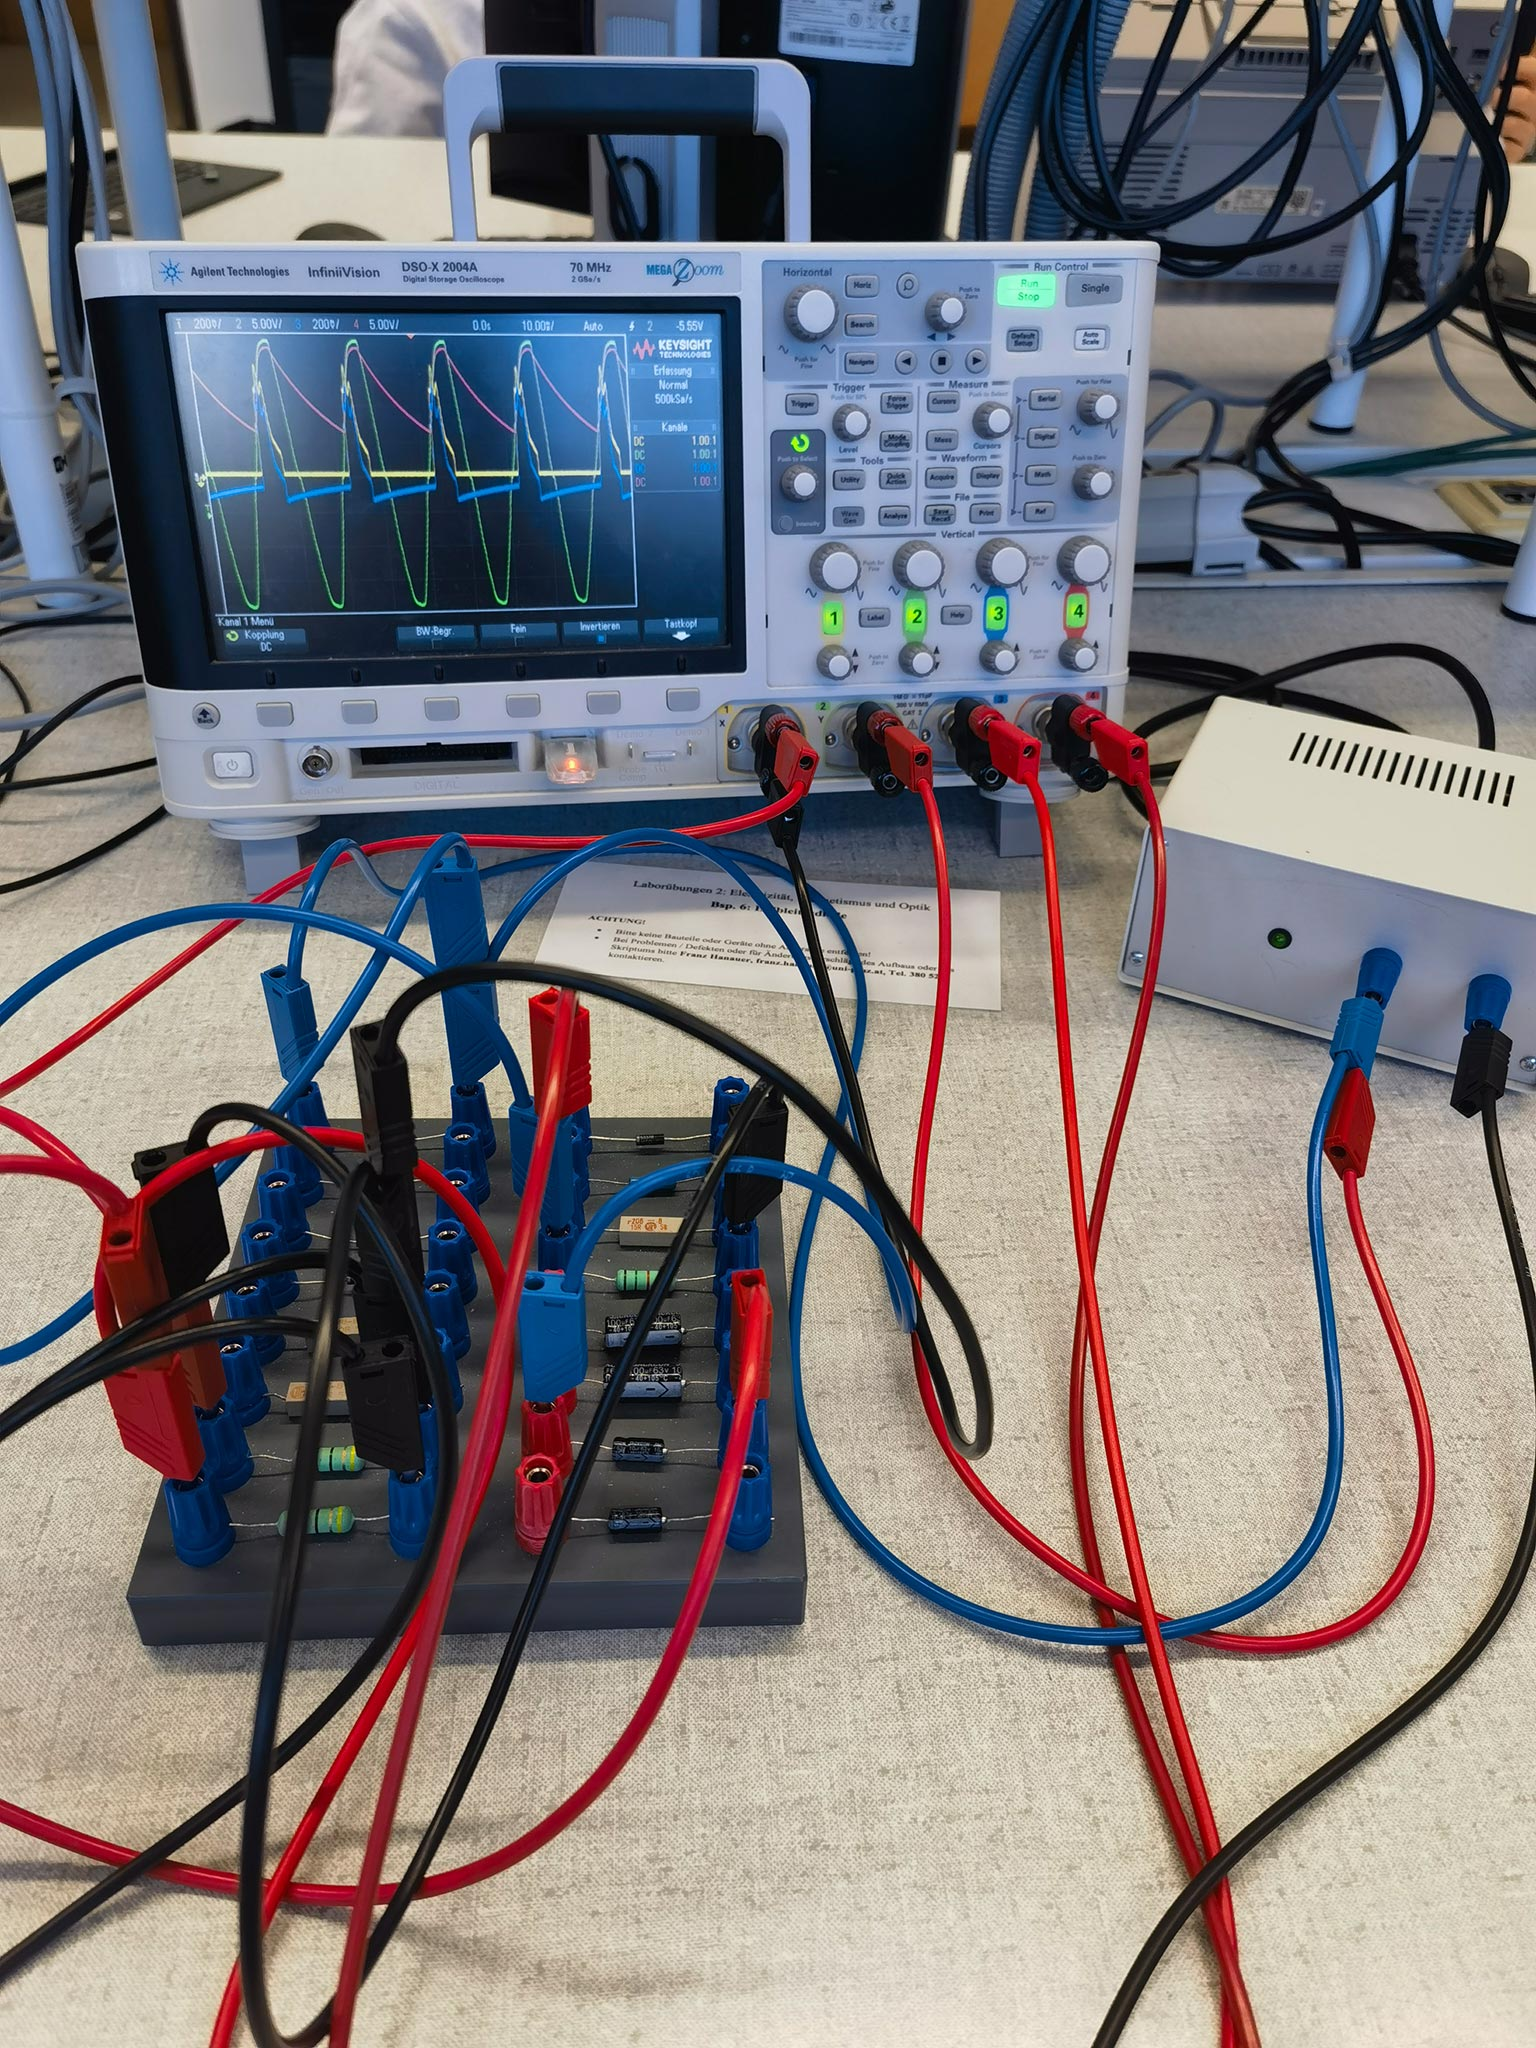
\includegraphics[width=0.4\linewidth]{nudes/3.jpg}
    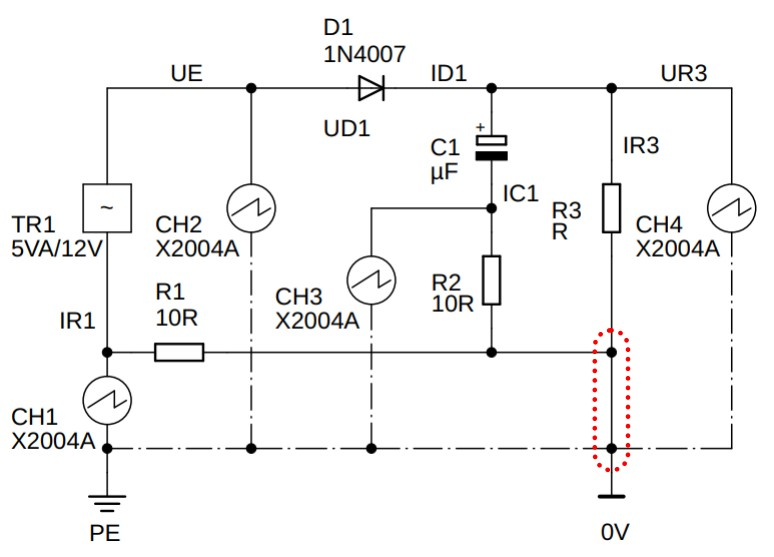
\includegraphics[width=0.4\linewidth]{nudes/aufbau3 schaltplan.jpg}
    \caption{Schaltbild (links) und Aufbau (rechts) Teil 3. Schaltbild entnommen aus Skriptum Halbleiterdiode Abbildung 1. \cite{teachcenter2}}
    \label{fig:aufbau 3}
\end{figure}

\section{Geräteliste} %jo holt a listn ------------------------------

    \begin{table}[H]
        \centering
        \caption{Im Versuch verwendete Geräte und Utensilien.}
        \label{tab:geraete}
        \begin{tabular}{| l | l | l | l |}
            \hline
            Gerät   & Typ   & Gerätenummer  & Unsicherheit \\
            \hline
        \end{tabular}
    \end{table}


\section{Versuchsdurchführung \& Messergebnisse} %nachvollziehbar und klar dargestellt ------------------------------


\section{Auswertung und Unsicherheitsanalyse} %Nicht nur zahlen angeben ------------------------------

In der Auswertung werden zur erhöhten Genauigkeit durchgehend ungerundete Werte bis zu den Endergebnissen verwendet und nur zur Darstellung gerundet. \\
Zur Berechnung der Unsicherheiten wird, wenn nicht anders angegeben, die Größtunsicherheitsmethode verwendet.


\section{Diskussion} %diskussion der Unsicherheiten und Ergebnisse und evtl. verlgeich mit Literatur ------------------------------


\section{Zusammenfassung} %klare, übersichtliche vollständige beantwortung der Aufgabenstellung ------------------------------


\printbibliography[heading=bibintoc]
\end{document}
